% Chapter 1

\chapter{Introduction} % Main chapter title

\label{Chapter1} % For referencing the chapter elsewhere, use \ref{Chapter1} 

% \lhead{Chapter 1. \emph{Introduction}} % This is for the header on each page - perhaps a shortened title

\graphicspath{{./Pictures/}}

%----------------------------------------------------------------------------------------
\section{Discovery and brief history}
\label{sec:Discovery and brief history}
Minute virus of mice (MVM) is a small, non-enveloped autonomous replicating parvovirus. Nowadays, two variant forms of MVM, that share 96 \% nucleotide sequence identity \cite{pmid3855242}, have been discovered independently. 
First, MVMp, the prototype strain, was isolated and characterized by Crawford in 1966. It originated from a contaminated murine adenovirus stock and was shown to replicate efficiently in mouse fibroblasts \cite{pmid5945715}. The virus was plaque purified in 1972 \cite{pmid4673484} and the resulting strain was designated MVM(p) for prototype \cite{MVMp}. Secondly, another strain was recovered from the culture fluid of infected murine EL-4 T-cell lymphoma cells by Bonnard and colleagues in 1976 \cite{pmid1244418}. This strain efficiently replicates in lymphocytes and is immunosuppressive for allogeneic mixed leukocyte cultures as it inhibits the generation of cytolytic T lymphocytes \cite{pmid6457871}. Therefore, it was referred to as immunosuppressive strain MVMi \cite{pmid6264106}. Both strains are well characterized and reciprocally restricted for growth in each other’s murine host cell.  

Since its discovery nearly 50 years ago, MVM served as an interesting model virus to dissect the molecular mechanisms of tissue tropism, capsid dynamics associated with endosomal trafficking, as well as viral DNA replication and packaging. Furthermore, it gained increasing interest as an important tool for cancer therapy due to its oncolytic capabilities and currently represents a commonly accepted parvovirus model.     


\section{Physicochemical properties}
Infectious parvovirus virions are composed of about 75 \% protein and 25 \% DNA. Their molecular weight is approximately 5.5-6.2 x 10\textsuperscript{6} Da. The virion buoyant density is 1.39 to 1.43 gcm\textsuperscript{-3}, measured in CsCl gradients \cite{CsCl, pmid4317344}. Since parvoviruses are devoid of a lipid envelope, mature virions are stable in the presence of lipid solvents. In particular, animal parvoviruses show considerable heat resistance. Most species remain stable and infectious on exposure to pH 7-9 or incubation at 56 \textcelsius~ for 60 min \cite{pmid12935806, pmid12385412, pmid17880601, pmid19039515}. Only harsh conditions, such as treatment with formalin, $\beta$-propiolacetone, hydroxylamine, ultraviolet light, and oxidizing agents as for example sodium hypochlorite ensure effective virus inactivation \cite{pmid4213983, pmid3416941, pmid7848502, pmid1520981}.    


\section{Morphology}
\label{sec:Morphology}

Parvoviruses belong to the smallest of isometric viruses. A linear single-stranded DNA genome of about 5 kb is packaged into the virus capsid \cite{pmid4975639, pmid5264145, pmid5429749}. They are non-enveloped and their diameters range from 215 \r{A} (Penaeus stylirostris densovirus, PstDNV) to 255 \r{A} (CPV) \cite{pmid10497831, icvt}. 

The icosahedral nature of parvoviruses was shown unambiguously by a combination of electron microscopy and, latterly, X-ray crystallography \cite{pmid2006420}. Interpretation of the structural data gave rise to three distinct types of surface topology among parvoviruses (see figure~\ref{Morphology}, p.~\pageref{Morphology}) \cite{pmid15795290}. The icosahedral twofold axes and the protrusions surrounding the icosahedral threefold axes display profound surface topology differences between each group. Types I and III comprise members of the \textit{Parvovirinae} subfamily described in section~\ref{sec: The Parvovirinae subfamily}, see p.~\pageref{sec: The Parvovirinae subfamily}. Members of the genus \textit{Protoparvovirus}, as for example CPV, FPV, MVM, and PPV, represent the first topology group that is characterized by a single, relatively flat, pinwheel-shaped protrusion at the icosahedral threefold axes and a wider twofold dimple. In comparison with the vertebrate parvoviruses, no large surface protrusions or depressions are present in \textit{Densovirus} capsids that appeared to be relatively spherical and featureless, adopting a second topology group \cite{pmid15769470, pmid9817847}. The third topology group encompasses the AMDV, B19V, AAV2, AAV4, and AAV5 capsids, which show three distinct mounds at a distance of $\sim$20-26 \r{A} from the icosahedral threefold axes. In addition, the depression at the twofold axis appears to be slightly deeper, particularly for B19V \cite{pmid20375175, pmid12136130, tropism}.        

\begin{figure}[h] 
\centering
\includegraphics[width=0.9\textwidth]{Morphology}
\caption[Parvovirus surface topology groups]{Surface topology groups among members of the \textit{Parvoviridae} family. Stereo, depth cued (blue-red-yellow-white) capsid surface illustration of representative members of the two subfamilies of the parvoviruses. Type viruses representing the three surface topology groups (I-III) and the genus to which they belong are indicated. A viral asymmetric unit bound (white triangle) is shown by a 2-fold (2f), two 3-folds (3f) and a 5-fold (5f) axis on the GmDNV image. A horizontal scale bar (100 \r{A}) for diameter measurement and a vertical color bar depicting color cueing as a function of particle radius in \r{A} are shown on the right hand side. These images were computed from atomic coordinates using the UCSF-Chimera program \cite{pmid15264254}, and all are rendered at the same resolution (7.9 \r{A}) and magnification. The figure was adapted from \cite{pmid20375175}.}
\label{Morphology}
\end{figure}

%The capsid surface of some, particularly invertebrate, parvoviruses appears to be smooth (Galleria mellonella densovirus, GmDNV) whereas others (Adeno-associated virus-2, AAV-2) are spiky at the 3- or 5-fold symmetry axes \cite{pmid10497831, icvt}.      


\nomenclature{PstDNV}{Penaeus stylirostris densovirus}
\nomenclature{GmDNV}{Galleria mellonella densovirus}
\nomenclature{DNA}{Deoxyribonucleic acid}


\section{Taxonomy}
\label{sec:Taxonomy}
The classification of the \textit{Parvoviridae} family is based on morphological and functional characteristics. Parvoviruses are ubiquitous pathogens that belong to the smallest DNA-containing viruses. Hence, the prefix "parvum" that means small in Latin. The name "parvovirus" was first introduced to the literature by Carlos Brailovsky, in an early attempt to establish a latinized binomial taxonomy system for viruses, in 1966 \cite{pmid5902774}. The age of the \textit{Parvoviridae} family may exceed 40 to 50 million years \cite{pmid20861255}. Apart from their ancient history, the genomes of parvoviruses were affirmed to display similar high mutation rates to RNA viruses \cite{pmid1649336, pmid12716974, pmid10411508, pmid16537636, pmid15626758, pmid21795474}. Such high mutation rates in conjunction with the long history might be a reason for the vast genetic divergence and extensive diversity seen within the \textit{Parvoviridae} family.      
The \textit{Parvoviridae} family comprises of non-enveloped, isometric viruses that contain linear single-stranded DNA genomes. Indeed, parvoviruses are the only viruses in the known biosphere that have both single-stranded and linear DNA genomes. The encapsidated single genomic molecule is 4-6 kb in length and terminates in palindromic duplex hairpin telomers. In general, there are two large open reading frames, ORF1 and ORF2, encoding for the non-structural protein(s) and the capsid protein(s), respectively. In some cases, an additional ORF3 has been identified that encodes an accessory protein, such as NP1, a non-structural protein only found in members of the genus \textit{Bocaparvovirus} and in PPV4 a member of the genus \textit{Copiparvovirus} \cite{pmid6319731, pmid21049037, pmid20339886}. As a consequence of such a simple genome, parvoviruses are highly dependent on their host for diverse functions in their reproduction \cite{pmid3296697, pmid10497831}. The terminal hairpins are fundamental for the unique replication strategy of the \textit{Parvoviridae} family and serve as an invariant hallmark for classification.
Members of the family \textit{Parvoviridae} infect a wide variety of hosts, ranging from insects to primates.
Depending on their host range, the \textit{Parvoviridae} are subdivided into \textit{Parvovirinae} infecting vertebrates and \textit{Densovirinae} infecting insects and other arthropods, respectively. The \textit{Parvovirinae} subfamily is further subdivided into eight genera: \textit{Amdoparvovirus}, \textit{Aveparvovirus}, \textit{Bocaparvovirus}, \textit{Copiparvovirus}, \textit{Dependoparvovirus}, \textit{Erythroparvovirus}, \textit{Protoparvovirus}, and \textit{Tetraparvovirus} (see figure~\ref{Fig: Taxonomy}, p.~\pageref{Fig: Taxonomy}) \cite{pmid24212889}. The subdivision into the eight genera is based on differences in transcription maps, organization of the ITRs, the ability to replicate efficiently either autonomously or with helper virus, the sense of the ssDNA that is packaged into separate virions, and sequence homology amongst the \textit{Parvovirinae} subfamily \cite{pmid11222696, icvt}.

\nomenclature{RNA}{Ribonucleic acid}

\begin{figure}[h]
\centering
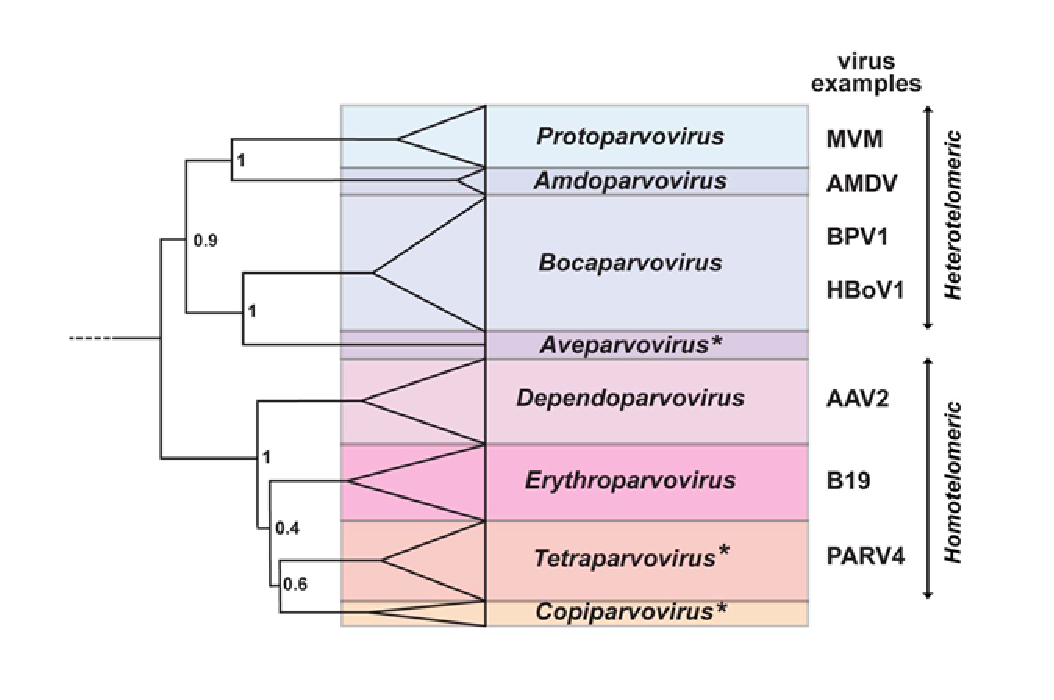
\includegraphics[width=\textwidth]{Taxonomy}
\caption[The \textit{Parvovirinae} subfamily]{The \textit{Parvovirinae} subfamily. The genera of the \textit{Parvovirinae} subfamily are depicted in a phylogenetic tree. Phylogenetic analysis is based on the amino acid sequence of the non-structural protein, NS1. The size of the color block for each genus indicates the relative number of species currently recognized, as an indicator of its diversity. Asterisks denote the names of new genera.} 
\label{Fig: Taxonomy}
\end{figure}



\subsection{The \textit{Parvovirinae} subfamily}
\label{sec: The Parvovirinae subfamily}   


\subsubsection{\textit{Amdoparvovirus}}

Mature virions exclusively contain negative strand genomic DNA of approximately 4.8 kb in length harbouring dissimilar palindromic sequences at each end \cite{pmid6252342, pmid2843669}. A single promoter located at map unit 3 at the left end of the genome generates all mRNA transcripts of AMDV. Polyadenylation may occur at either the proximal site or at the distal site of the genome. Thus, the transcription profile of the genus \textit{Amdoparvovirus} most closely resembles  that of the genus \textit{Erythroparvovirus} \cite{pmid16378968}.  
Only two distant species have been reported. Firstly, \textit{Carnivore amdoparvovirus 1}, which comprises only Aleutian mink disease virus (AMDV) and secondly, \textit{Carnivore amdoparvovirus 2}, which encompasses solely gray fox amdovirus (GFAV) \cite{pmid22000359}. 
Permissive replication is tightly restricted to Crandell feline kidney cells. The virion surface displays three mounds elevated around the threefold icosahedral axis of symmetry. Several structure features were ascertained to be similar to those found in B19V, CPV, FPV, and MVM. Such appearance is comparable to those observed for the genus \textit{Dependoparvovirus} \cite{pmid10400786}. Remarkably, there is no evidence of a phospholipase 2A enzymatic core within the naturally truncated N-VP1 terminus of members belonging to the genus \textit{Amdoparvovirus} as it is common to the other genera of the subfamily \textit{Parvovirinae} \cite{icvt}. 


\nomenclature{AMDV}{Aleutian mink disease virus}
\nomenclature{GFAV}{Gray fox amdovirus}
\nomenclature{PLA\textsubscript{2}}{Phospholipase A2}

\subsubsection{\textit{Aveparvovirus}}

\textit{Aveparvovirus} is a new genus within the \textit{Parvovirinae} subfamily that comprises of the species chicken parvovirus and turkey parvovirus. The name \textit{Aveparvovirus} is derived from \underline{av}ian parvoviruses, referring to the hosts from which the members were isolated. Although these viruses were identified for years in the intestinal tracts of poultry \cite{pmid18766849, pmid6847550, pmid2995561}, analysis of the complete nucleotide sequence has been reported only recently. Phylogenetic study of the genomic sequences revealed that interestingly, ChPV and TuPV do not group phylogenetically with GPV and DPV, that are members of the genus \textit{Dependoparvovirus}. It was clearly demonstrated that ChPV, along with the closely related TuPV, represents the prototype of a novel genus within the \textit{Parvovirinae} subfamily \cite{pmid25510852, pmid18622862}. Identical direct repeat sequences flank the genome at both the 3' and the 5' end. Each of which contains a 39 nt ITR that is predicted to form a hairpin structure. ChPV and TuPV feature an overall genome organization similar to that of members of the genus \textit{Bocaparvovirus} \cite{pmid20097398}. 
Although it has been demonstrated that ChPV can induce clinical signs in broiler chickens that show characteristics of the runting-stunting syndrome (RSS) \cite{pmid18766892}, the role of avian parvoviruses in the aetiology of enteric diseases in poultry still remains to be demonstrated. RSS, also referred to as malabsorption syndrome, is characterized by significantly decreased egg hatchability, poorly developed hatched chickens, serious growth retardation, diarrhoea, enteritis, disturbed feathering, low vitality, and bone disorders \cite{pmid7150147, pmid6281962, pmid8363509}. Currently, the pathogenicity of TuPV has not been investigated yet. The predominant enteric diseases in turkeys are known as poult enteritis complex (PEC) \cite{pmid10935280} or the more drastic poult enteritis mortality syndrome (PEMS) \cite{PEMS}. Understanding the role of avian parvoviruses in PEMS, PEC, and RSS is of great interest due to the economic losses resulting from enteric diseases in poultry. \cite{pmid18622862}. 
  
    



\nomenclature{ChPV}{Chicken parvovirus}
\nomenclature{TuPV}{Turkey parvovirus} 
\nomenclature{GPV}{Goose parvovirus}
\nomenclature{DPV}{Duck parvovirus}
\nomenclature{RSS}{Runting-stunting syndrome}
\nomenclature{PEC}{Poult enteritis complex}
\nomenclature{PEMS}{Poult enteritis mortality syndrome}


\subsubsection{\textit{Bocaparvovirus}}
The name of the genus is derived from \underline{bo}vine and \underline{ca}nine, referring to the two hosts of the first identified members of this genus.  The genomes of members of the genus \textit{Bocaparvovirus} are quite distinct from all other viruses in the subfamily \textit{Parvovirinae}. As the members of the genera \textit{Protoparvovirus} and \textit{Amdoparvovirus} they contain non-identical imperfect palindromic sequences at both ends of their 5.5 kb genome. Mature virions contain mainly, but not exclusively, negative strand ssDNA \cite{pmid3783814,pmid12441065}.
All RNA transcripts are generated from a single P4 promoter at the left-hand end of the genome. The transcripts are alternatively spliced and polyadenylated either at an internal site or at the 3’-end of the genome \cite{pmid17715221}. Noteworthy, bovine parvovirus (BPV), the main representative, encodes a 22.5 kDa nuclear phosphoprotein, NP1, whose function still remains unknown. This protein is distinct from any other parvovirus-encoded polypeptide \cite{pmid6319731}.
A human bocavirus was first described in 2005, when it was detected in nasopharyngeal aspirates of young children with respiratory tract infection \cite{pmid11562506, pmid16118271}. More recently, HBoV has been identified in diarrheal feces of children with gastroenteritis \cite{pmid17553287}. HBoV infection is associated with acute respiratory symptoms and is usually detected in children under 2 years of age \cite{pmid17122013, pmid16517912, pmid17041855}. HBoV infections have been reported world-wide and HBoV was often isolated in respiratory samples of diseased as well as asymptomatic patients sometimes long after the primary infection. Therefore, it can be frequently detected even though it is not likely acting as a pathogen, thus complicating the use of PCR in diagnostics. Furthermore, long-term persistence may explain that HBoV infection among adults was predominantly reported in association with immunosuppression or immunodeficiency \cite{pmid17041855, pmid17176591}.         



\nomenclature{BPV}{Bovine parvovirus}
\nomenclature{kDa}{Kilodalton}
\nomenclature{Da}{Dalton}


\subsubsection{\textit{Copiparvovirus}}
Based on phylogenetic analysis, the genus \textit{Copiparvovirus} encompasses PPV4 and BPV2. PPV4 was identified in clinical samples from swine herds \cite{pmid20339886, pmid21092136, pmid22967311} and represents a distinct branch together with BPV2 \cite{pmid11562506}. The name \textit{Copiparvovirus} refers to \underline{co}ws and \underline{pi}gs, the hosts from which members of that genus were isolated. PPV4 is unique in that it is phylogenetically most closely related to BPV2 but the coding capacity and genome organization resemble more those of viruses of the genus \textit{Bocaparvovirus}. While the ORF3 encoded proteins of the three recognized \textit{Bocaparvovirus} members share amino acid identities of 43.3-47.0 \% among themselves, the PPV4 ORF3 encoded protein does not display homology with any protein in the GenBank database \cite{pmid20339886, pmid21092136}. 
Recently, two novel porcine parvoviruses, PPV5 and PPV6, were discovered \cite{pmid23405295, pmid25442288}. Characterization of their nucleotide sequences revealed that their full-length genomes are approximately 6 kb in length. As a consequence of this capacious genome size, especially their capsid protein encoding genes are exceptionally large. Interestingly, the genomic organization of PPV5 and PPV6 is different from PPV4 in that they lack the extra ORF3 in the middle of the genome. Moreover, PPV5 as well as PPV6 possess the conserved putative secretory PLA\textsubscript{2} motif which is present in the capsid protein of most parvoviruses but is lacking in PPV4. In spite of considerable differences in the genomic organization between BPV2, PPV5, and PPV6 on the one hand and PPV4 on the other hand, phylogenetic analysis revealed a close evolutionary relationship of these viruses, suggesting that they share the same immediate ancestor \cite{pmid23762339, pmid25442288}.      
Since members of the genus \textit{Copiparvovirus} were discovered quite recently, their biological characteristics, relatedness to disease, and potential clinical manifestations are still not fully understood \cite{pmid20339886, pmid21092136, pmid23762339, pmid25442288}. Especially, Kresse strain of porcine parvovirus belonging to the genus \textit{Protoparvovirus} is known to be an important pathogen responsible for embryonic and fetal death in piglets, resulting in considerable losses in the pig industry worldwide \cite{pmid6314634, pmid427636, pmid999067, pmid3006323}. In order to clarify the precise role of the most recently discovered members of the genus \textit{Copiparvovirus} as causative agents of reproductive failure in breeding animals, more comprehensive epidemiologic studies are required in the future \cite{pmid25442288}. 



\subsubsection{\textit{Dependoparvovirus}}
Positive and negative strand ssDNA is distributed indifferently among mature virions belonging to the genus \textit{Dependoparvovirus} \cite{pmid5014934, pmid5264145}. The 4.7 kb DNA molecule contains identical ITRs of 145 nt, the first 125 nt of which form a palindromic sequence \cite{pmid6246271}. Three mRNA promoters that are located at map units 5, 19, and 40 initiate transcription that can be terminated in two polyadenylation sites located at the right-hand end or alternatively, in the middle of the genome \cite{pmid6253077, pmid6281463}. Common for all currently accepted replication-defective members of the genus \textit{Dependoparvovirus} is their strict dependence upon helper adenoviruses or herpesviruses \cite{pmid4318977, pmid6270377, pmid5227666}. Therefore, their host range tropism strongly depends on the one of the helper virus. 
The only exceptions are the autonomously replicating duck and goose parvoviruses which are also comprised within the \textit{Dependoparvovirus} genus based on phylogenetic analysis \cite{icvt}. The most important members of this genus are the adeno-associated viruses (AAV). They attracted considerable interests since at least one of them, AAV-2, has been reported to integrate site-specifically into human chromosome 19 \cite{pmid2156265, pmid1653762, pmid1334463, pmid1657596}. This characteristic makes AAV a promising candidate for creating viral vectors for gene therapy \cite{pmid18854481, pmid21499295}. As a well characterized member of the \textit{Dependoparvoviruses} AAV-2 represents the model virus among this genus.  


\subsubsection{\textit{Erythroparvovirus}}
Equivalent numbers of positive and negative sense ssDNA are packaged into infectious virions of the genus \textit{Erythroparvovirus}. As in the case with the genus \textit{Dependoparvovirus}, the 5.5 kb ssDNA molecule contains identical ITRs of 383 nt in length at both the 3’ and the 5’ end. The first 365 nt of those secondary elements form palindromic sequences \cite{pmid2408228}. Transcription is regulated by a single mRNA promoter located at map unit 6 \cite{pmid3824910}. A distal polyadenylation site for use in termination of RNA synthesis is located at the far right side. Additionally, transcripts may be terminated at an unusual internal polyadanylation site in the middle of the genome \cite{pmid3599180}. Viruses belonging to this genus are highly erythrotropic, meaning that efficient replication only occurs in rapidly dividing erythroid progenitor cells (EPCs) such as erythroblasts and megakaryocytes present in the bone marrow.
B19V, a widespread human pathogen that causes fifth disease, polyarthropathia, anemic crises in children with underlying hematological diseases (e.g. sickle cell anemia or thalassemia) and intrauterine infections (with hydrops fetalis in some cases) \cite{pmid12097253} represents the model virus among the genus \textit{Erythroparvovirus}. 

\nomenclature{Nt}{Nucleotide}
\nomenclature{ITR}{Inverted terminal repeat}
\nomenclature{Kb}{Kilo base}
\nomenclature{EPC}{Erythroid progenitor cell}


\subsubsection{\textit{Protoparvovirus}}
Kilham Rat virus (KRV), a member of the genus \textit{Protoparvoviruses} was the first member of the subfamily \textit{Parvovirinae} to be discovered in 1959 \cite{pmid13669314}. Some members of the genus contain positive strand DNA in variable proportions up to 50 \% \cite{pmid6694260}. However, in mature virions of most members, virtually only negative strand DNA occurs. What they have in common are their hairpin structures at both the 5’ and 3’ ends of the linear 5 kb ssDNA molecule that differ in both sequence and predicted structure \cite{pmid6298737}. Transcription of the genome is regulated by two mRNA promoters at map units 4 and 39 \cite{pmid6828378}. There is only one polyadenylation site at the 3’ end. 
Viral replication provokes characteristic cytopathic effects in cell culture. Many species display hemagglutination with erythrocytes of one or several species, but not enforcedly of their natural host \cite{pmid5083410}. The genus \textit{Protoparvovirus} is primarily represented by MVM \cite{icvt, protoparvovirus}.       

\nomenclature{KRV}{Kilham rat virus}

\subsubsection{\textit{Tetraparvovirus}}
The genus \textit{Tetraparvovirus} is a new genus that arose recently. To date, six species have been discovered, which were isolated from humans \cite{pmid15956568}, chimpanzees, baboons \cite{pmid20668071}, cows, pigs \cite{pmid18632954, pmid20653980, pmid22247522}, as well as sheep \cite{pmid21980506}. RNA transcripts that encode the NS-proteins or the VP-proteins are generated from two promoters that are located at map units 6 and 38, respectively. Transcription can be terminated in two polyadenylation sites located at the right-hand end of the genome or alternatively, at an internal polyadenylation site. Since the full-length genome has not been sequenced yet, information of the terminal repeats is still lacking \cite{pmid22044541}. Analysis of the NS1 protein revealed a G2/M cell cycle arrest induced in NS1-expressing hematopoietic stem cells that clearly involved the predicted helicase motifs \cite{pmid8106366, pmid9261429, pmid7966641} of NS1. To date, no PLA\textsubscript{2}-like activity of expressed VP1u polypeptides has been demonstrated for any member of the genus \textit{Tetraparvovirus} \cite{pmid22044541}. PARV4 is one of the only four groups of parvoviruses that is known to infect humans besides B19V, HBoV, and AAV. It was first reported in an intravenous drug user who was positive for HBV infection in 2005. The patient suffered from arthralgia, confusion, diarrhea, fatigue, neck stiffness, night sweat, pharyngitis, and vomiting. PARV4 represents a phylogenetic deeply rooted lineage between avian dependoviruses and bovine parvovirus type 3 \cite{pmid15956568}. So far, most evidence about PARV4 transmission comes from patients who had engaged in high risk behaviour for blood borne viral infections, where PARV4 infection basically was observed to be strongly associated with HCV and HIV infection \cite{pmid22492853, pmid22235298, pmid17397006}. However, there are several reports of parenteral transmission in the absence of HIV, HBC, or HCV. PARV4 IgG has been documented independently from other blood borne viruses among injecting drug users \cite{pmid23283958}, in haemophilia patients \cite{pmid22043925}, and in patients who were subjected to intra-muscular injections in the past \cite{pmid22469425}. Currently, no definitive clinical syndrome was associated with PARV4 infection and there is no evidence for a potential pathogenicity of related members of the genus \textit{Tetraparvovirus} in animals \cite{pmid18632954}. PARV4 viraemia appears to be asymptomatic \cite{pmid20587191} and co-existing blood borne viruses do not increase severity \cite{pmid22235298}.   

  








 


\nomenclature{PARV4}{Parvovirus 4}
\nomenclature{HBoV}{Human Bocavirus}
\nomenclature{HIV}{Human immunodeficiency virus}
\nomenclature{HCV}{Hepatitis C virus}
\nomenclature{HBV}{Hepatitis B virus}
\nomenclature{ORF}{Open reading frame}
\nomenclature{VP1u}{VP1 unique region}

\clearpage



\begin{tiny}
\begin{center}

\begin{longtable}{p{0.7in} p{1.65in} p{1.6in} p{0.6in} p{0.65in}}
\caption[Taxonomy for the subfamily \textit{Parvovirinae}]{Taxonomy for the subfamily \textit{Parvovirinae}}\\
\\
\label{Tab: Taxonomy}
\textbf{Genus} & \textbf{Species} & \textbf{Virus or virus variants} & \textbf{Abbr.} & \textbf{ACNO}\footnotemark\\
\hline
\endfirsthead % all the lines above this will be repeated on every page


\multicolumn{3}{l}{\textbf{Table~\ref{Tab: Taxonomy}} continued}\\
\\
\textbf{Genus} & \textbf{Species} & \textbf{Virus or virus variants} & \textbf{Abbr.} & \textbf{ACNO}\footnotemark\\
\hline
\endhead

\hline
\multicolumn{5}{l}{The type species for each genus is indicated in bold type. \cite{pmid24212889}}
\endlastfoot

\textit{Amdoparvovirus} & \textbf{\textit{Carnivore amdoparvovirus 1}} & Aleutian mink disease virus & AMDV & JN040434 \\
 & \textit{Carnivore amdoparvovirus 2} & Gray fox amdovirus & GFAV & JN202450 \\
\textit{Aveparvovirus} & \textit{\textbf{Galliform aveparvovirus 1}} & Chicken parvovirus & ChPV & GU214704 \\
& & Turkey parvovirus & TuPV & GU214706 \\
\textit{Bocaparvovirus} & \textit{Carnivore bocaparvovirus 1} & Canine minute virus & CnMV & FJ214110 \\
& \textit{Carnivore bocaparvovirus 2} & Canine bocavirus 1 & CBoV & JN648103 \\
& \textit{Carnivore bocaparvovirus 3} & Feline bocavirus & FBoV & JQ692585 \\
& \textit{Pinniped bocaparvovirus 1} & California sea lion bocavirus 1 & CslBoV1 & JN420361\\
& & California sea lion bocavirus 2 & CslBoV2 & JN420366 \\
& \textit{Pinniped bocaparvovirus 2} & California sea lion bocavirus 3 & CslBoV3 & JN420365 \\
 & \textit{Primate bocaparvovirus 1} & Human bocavirus 1 & HBoV1 & JQ923422 \\
 & & Human bocavirus 3 & HBoV3 & EU918736 \\
 & & Gorilla bocavirus & GBoV & HM145750 \\
 & \textit{Primate bocaparvovirus 2} & Human bocavirus 2a & HBoV2a & FJ973558 \\
 & & Human bocavirus 2b & HBoV2b & FJ973560 \\
 & & Human bocavirus 2c & HBoV2c & FJ170278 \\
 & & Human bocavirus 4 & HBoV4 & FJ973561 \\
 & \textit{\textbf{Ungulate bocaparvovirus 1}} & Bovine parvovirus & BPV & DQ335247 \\
 & \textit{Ungulate bocaparvovirus 2} & Porcine bocavirus 1 & PBoV1 & HM053693 \\ 
 & & Porcine bocavirus 2 & PBoV2 & HM053694 \\
 & & Porcine bocavirus 6 & PBoV6 & HQ291309 \\
 & \textit{Ungulate bocaparvovirus 3} & Porcine bocavirus 5 & PBoV5 & HQ223038 \\
 & \textit{Ungulate bocaparvovirus 4} & Porcine bocavirus 7 & PBoV7 & HQ291308 \\ 
 & \textit{Ungulate bocaparvovirus 5} & Porcine bocavirus 3 & PBoV3 & JF429834 \\ 
 & & Porcine bocavirus 4-1 & PBoV4-1 & JF429835 \\
 & & Porcine bocavirus 4-2 & PBoV4-2 & JF429836 \\
 \textit{Copiparvovirus} & \textit{\textbf{Ungulate copiparvovirus 1}} & Bovine parvovirus 2 & BPV2 & AF406966 \\
 & \textit{Ungulate copiparvovirus 2} & Porcine parvovirus 4 & PPV4 & GQ387499 \\
 \textit{Dependoparvovirus} & \textit{\textbf{Adeno-associated dependoparvovirus A}} & Adeno-associated virus-1 & AAV1 & AF063497 \\ 
 & & Adeno-associated virus-2 & AAV2 & AF043303 \\
 & & Adeno-associated virus-3 & AAV3 & AF028705 \\
 & & Adeno-associated virus-4 & AAV4 & U89790 \\
 & & Adeno-associated virus-6 & AAV6 & AF028704 \\
 & & Adeno-associated virus-7 & AAV7 & AF513851 \\
 & & Adeno-associated virus-8 & AAV8 & AF513852 \\
 & & Adeno-associated virus-9 & AAV9 & AX753250 \\
 & & Adeno-associated virus-10 & AAV10 & AY631965 \\ 
 & & Adeno-associated virus-11 & AAV11 & AY631966 \\ 
 & & Adeno-associated virus-12 & AAV12 & DQ813647 \\
 & & Adeno-associated virus-13 & AAV13 & EU285562 \\
 & & Adeno-associated virus-S17 & AAVS17 & AY695376 \\
 & \textit{Adeno-associated dependovirus B} & Adeno-associated virus-5 & AAV5 & AF085716 \\
 & & Bovine adeno-associated virus & BAAV & AY388617 \\
 & & Caprine adeno-associated virus & CapAAV & DQ335246 \\
 & \textit{Anseriform dependoparvovirus 1} & Duck parvovirus & DPV & U22967 \\
 & & Goose parvovirus-PT & GPV2 & JF926695 \\
 & & Goose parvovirus & GPV & U25749 \\
 & \textit{Avian dependovirus 1} & Avian adeno-associated virus & AAAV & AY186198 \\
 & \textit{Chiropteran dependoparvovirus 1} & Bat adeno-associated virus & BtAAV & GU226971 \\
 & \textit{Pinniped dependoparvovirus 1} & California sea lion adeno-associated virus & CslAAV & JN420372 \\
 & \textit{Squamate dependoparvovirus 1} & Snake adeno-associated virus & SAAV & AY349010 \\
 \textit{Erythroparvovirus} & \textit{\textbf{Primate erythroparvovirus 1}} & Human parvovirus B19-Au & B19V-Au & M13178 \\
 & & Human parvovirus B19-J35 & B19V-J35 & AY386330 \\
 & & Human parvovirus B19-Wi & B19V-Wi & M24682 \\
 & & Human parvovirus B19-A6 & B19V-A6 & AY064475 \\
 & & Human parvovirus B19-Lali & B19V-Lali & AY044266 \\
 & & Human parvovirus B19-V9 & B19V-V9 & AJ249437 \\
 & & Human parvovirus B19-D91 & B19V-D91 & AY083234 \\
 & \textit{Primate erythroparvovirus 2} & Simian parvovirus & SPV & U26342 \\
 & \textit{Primate erythroparvovirus 3} & Rhesus macaque parvovirus & RhMPV & AF221122 \\
 & \textit{Primate erythroparvovirus 4} & Pig-tailed macaque parvovirus & PtMPV & AF221123 \\
 & \textit{Rodent erythroparvovirus 1} & Chipmunk parvovirus & ChpPV & GQ200736 \\
 & \textit{Ungulate erythroparvovirus 1} & Bovine parvovirus 3 & BPV3 & AF406967 \\
 \textit{Protoparvovirus} & \textit{Carnivore protoparvovirus 1} & Feline parvovirus & FPV & EU659111 \\ 
 & & Canine parvovirus & CPV & M19296 \\
 & & Mink enteritis virus & MEV & D00765 \\
 & & Racoon parvovirus & RaPV & JN867610 \\
 & \textit{Primate protoparvovirus 1} & Bufavirus 1a & BuPV1a & JX027296 \\
 & & Bufavirus 1b & BuPV1b & JX027295 \\
 & & Bufavirus 2 & BuPV2 & JX027297 \\
 & \textit{\textbf{Rodent protoparvovirus 1}} & H-1 parvovirus & H1 & X01457 \\
 & & Kilham rat virus & KRV & AF321230 \\
 & & LuIII virus & LuIII & M81888 \\
 & & Minute virus of mice (prototype) & MVMp & J02275 \\
 & & Minute virus of mice (immunosuppressive) & MVMi & M12032 \\
 & & Minute virus of mice (Missouri) & MVMm & DQ196317 \\
 & & Minute virus of mice (Cutter) & MVMc & U34256 \\
 & & Mouse parvovirus 1 & MPV1 & U12469 \\
 & & Mouse parvovirus 2 & MPV2 & DQ196319 \\
 & & Mouse parvovirus 3 & MPV3 & DQ199631 \\
 & & Mouse parvovirus 4 & MPV4 & FJ440683 \\
 & & Mouse parvovirus 5 & MPV5 & FJ441297 \\
 & & Hamster parvovirus & HaPV & U34255 \\ 
 & & Tumor virus X & TVX & In preparation \\
 & & Rat minute virus 1 & RMV1 & AF332882 \\
 & \textit{Rodent protoparvovirus 2} & Rat parvovirus 1 & RPV1 & AF036710 \\
 & \textit{Ungulate protoparvovirus 1} & Porcine parvovirus Kresse & PPV-Kr & U44978 \\
 & & Porcine parvovirus NADL-2 & PPV-NADL2 & L23427 \\
 \textit{Tetraparvovirus} & \textit{Chiropteran tetraparvovirus 1} & Eidolon Helvum (bat) parvovirus & Ba-PARV4 & JQ037753 \\
 & \textit{\textbf{Primate tetraparvovirus 1}} & Human parvovirus 4 G1 & PARV4G1 & AY622943 \\
 & & Human parv4 G2 & PARV4G2 & DQ873391 \\      
 & & Human parv4 G3 & PARV4G3 & EU874248 \\
 & & Chipmanzee parv4 & Ch-PARV4 & HQ113143 \\
 & \textit{Ungulate tetraparvovirus 1} & Bovine hokovirus 1 & B-PARV4-1 & EU200669 \\
 & & Bovine hokovirus 2 & B-PARV4-2 & JF504697 \\
 & \textit{Ungulate tetraparvovirus 2} & Porcine hokovirus & P-PARV4 & EU200677 \\
 & \textit{Ungulate tetraparvovirus 3} & Porcine Cn virus & CnP-PARV4 & GU938300 \\
 & \textit{Ungulate tetraparvovirus 4} & Ovine hokovirus & O-PARV4 & JF504699 \\
 



\label{Taxonomy for the subfamily Parvovirinae}
     
\end{longtable}
\end{center} 
\end{tiny}



\footnotetext{NIH GenBank accession number}
\nomenclature{NIH}{National institutes of health}

\newpage

\section{Tissue Tropism and Pathogenicity Determinants}
Concerning their host range, most parvoviruses, such as MVM, \nomenclature{MVM}{Minute virus of mice} CPV, \nomenclature{CPV}{Canine parvovirus} and FPV, \nomenclature{FPV}{Feline parvovirus} are tightly restricted to specific receptors of their particular hosts. However, some parvoviruses, as for example many of the AAVs, \nomenclature{AAV}{Adeno-associated virus} infect human cells by primary attachment to a variety of receptors. 

As outlined in section~\ref{sec:Discovery and brief history} (see p.~\pageref{sec:Discovery and brief history}), two distinct strains of the parvovirus MVM have been described to occur in mice. On the one hand, MVMp, \nomenclature{MVMp}{Prototype strain of MVM} the prototype strain, replicates efficiently in mouse fibroblasts \cite{pmid5945715}. On the other hand, MVMi,\nomenclature{MVMi}{Immunosuppressive strain of MVM} the immunosuppressive strain, replicates in T lymphocytes \cite{pmid1244418}.
Both strains display disparate \textit{in vitro} tropism and \textit{in vivo} pathogenicity despite differing by only 14 amino acids in their capsid proteins \cite{pmid1871965}. Beyond that, MVMp and MVMi are serologically indistinguishable, bind to sialic acid and are internalized in both fibroblasts and lymphocytes \cite{pmid6602221}. Consequently, it could be demonstrated that both viruses propagate in hybrids of the two cell types \cite{pmid6602222}.    

In order to map the allotropic determinants of MVM, chimeric viral genomes were constructed \textit{in vitro} from infectious genomic clones of both strains. By mutagenesis and selective plaque assays, the major determinants for the acquisition of fibrotropism for MVMi have been mapped onto the capsid \cite{pmid3257270, pmid9519837, pmid1871965}, in particular to the VP2 residues 317 and 321 \cite{pmid7637028, pmid1316457}. Both residues are located at the base of the threefold spike of the virion \cite{pmid3357208, pmid3392768, pmid3257270}. Interestingly, these two VP2 residues structurally localize nearby some of the important amino acids determining CPV, FPV, and PPV host range \cite{pmid14581558, pmid12941920, pmid1532105}. Further residues (VP2 residues 399, 460, 553, and 558) were identified in MVMi to be able to confer fibrotropism to forward second-site mutants when either residues 317 or 321 are mutated. Those residues cluster around the twofold dimple-like depression \cite{pmid9817841}. In contrast, the switch to lymphotropism for MVMp is more complex and requires both an equivalent region of the major MVMi capsid protein gene VP2 and a segment of the nonstructural protein genes \cite{pmid9519837}.    

MVMi appears to be more pathogenic in mice than MVMp. Oronasal inoculation of MVMi in most neonatal mice resulted in lethal phenotype or severe growth-retardation in survivors \cite{pmid3712557}, as observed for other parvoviruses (see section~\ref{sec: The Parvovirinae subfamily}, p.~\pageref{sec: The Parvovirinae subfamily}). MVMp infection appears to be asymptomatic in newborn mice \cite{pmid1373202}. In contrast, MVMi infection in neonatal mice of some inbred strains caused renal papillary hemorrhage and viral replication in endothelia \cite{pmid1653878}, hematopoietic precursors \cite{pmid7707557}, and neuroblasts \cite{pmid8892936}. Following \textit{in utero} inoculation of MVMi or MVMp into developing embryo, a broad set of cell types were infected that partially overlapped. Nevertheless, the tissue tropism of MVMp for fibroblasts and of MVMi for endothelium, as well as the higher virulence of MVMi was preserved \cite{pmid15308740}. 
By reason of the complexity of MVMi pathogenesis in the neonatal mouse, a more adequate model was required to investigate the virulence of MVMi \textit{in vivo}. 

Severe combined immunodeficiency (SCID) mice \cite{pmid6823332} represent such a model since they lack an antigen-specific immune response, thus allowing the study in adult mice and circumventing the complex situation of heterogenous viral multiplication in embryonic developing tissue. MVMi infection of adult SCID mice gave rise to the suppression of long-term repopulating hemopoietic stem cells in the bone marrow \cite{pmid12857918}, leading to an acute lethal leukopenia and accelerated erythropoiesis \cite{pmid9971754}.
In addition, it has been reported that MVMp evolved in intravenously inoculated SCID mice. Different variants, isolated from single plaques, carried only one of three single amino acid changes at position 325, 362, or 368 in the major VP2 capsid protein. These variants sustained their fibrotropism \textit{in vitro}, but unlike MVMp, they propagated in mouse tissues following oronasal inoculation, eventually causing death \cite{pmid16415031, pmid16103180}.
Two of the three invasive fibrotropic MVMp strains, I362S and I368R, were shown to induce lethal leukopenia in oronasal inoculated SCID mice. Emerging viral populations in leukopenic mice displayed altered sequences in the MVMi genotype at position 321 and 551 of VP2 for infections with the I362S variant or changes at position 551 and 575 in the K368R virus infections. In general, a high level of genomic heterogeneity in the DNA sequence encoding the VP2 protein was observed and was found to be clustered at the twofold depression of the viral capsid \cite{pmid18045943}.            	
	
	
	Significantly, the amino acids dictating \textit{in vitro} tropism (317 and 321), \textit{in vivo} pathogenicity (325, 362, and 368), fibrotropism on MVMi (399, 460, 553, and 558), and those involved in the development of leukopenia (321, 551, and 575) were found to be located on, or near the capsid surface. Structurally, these residues cluster mainly by raised elements around the twofold axes of symmetry, in close vicinity of the sialic acid binding pocket \cite{pmid16415031, pmid18045943}.   
	
Differences in the tissue tropisms and the pathogenic phenotypes  have also been mapped to the capsid proteins of Aleutian mink disease parvovirus \cite{pmid8396664}, porcine parvovirus (PPV) \nomenclature{PPV}{Porcine parvovirus} \cite{pmid8642680}, CPV \cite{pmid3176341, pmid1331498}, and FPV \cite{pmid7513918} in a capsid region analogous to that observed for MVM (reviewed in \cite{tropism}). These pronounced \textit{in vitro} tropism and \textit{in vivo} pathogenicity disparities between the highly homologous viruses can occur at any of the various stages of the infectious viral life cycle, including cell receptor binding, internalization, capsid uncoating, DNA replication or transcription. Although the same structural elements of viruses are involved in mediating host and tissue tropisms, each appears to be affecting a different mechanism. Host ranges of CPV and FPV are controlled by receptor binding, whereas the cell tropisms of MVM appear to be due to restrictions of interactions with intracellular factors \cite{pmid9817841, pmid12941411, pmid6602221}. For MVM it was suggested that the point of restriction appeared after nuclear targeting and conversion of genomic ssDNA to RF intermediates but prior to viral genome replication. Most likely, the restraint occurs due to a block in capsid uncoating \cite{pmid9311862, pmid1322591}.

As discussed in this section the functional regions among the subfamily \textit{Parvovirinae} co-localize to similar capsid surface regions albeit three general parvovirus topology groups with characteristic local morphological surface differences emerged (see section~\ref{sec:Morphology}, p.~\pageref{sec:Morphology}). A profound understanding of functional domains that are involved in fundamental steps of the viral life cycle, particularly receptor attachment, \textit{in vitro} tropism, \textit{in vivo} pathogenicity, and antigenicity are essential for infection and disease control. Hence, showing great promise to allow genetic engineering of parvovirus capsids for the therapeutic delivery to be controlled or modified in gene therapy applications and to develop foreign antigens \cite{pmid12941411, tropism}.     



%Although MVMi infection may result in pathology of infected mice, it has been shown that the infection more likely interferes with numerous T-cell functions \textit{in vitro}. The infection rather causes problems for the ongoing study the mice are being used for as the immune system will be activated, the activity of T-lymphocytes or B-lymphocytes will be altered and tumor formation may be suppressed \cite{pmid6457871, pmid6264106, pmid11528091}.

\nomenclature{SCID}{Severe combined immunodeficiency}
\nomenclature{RF}{Replicative form}
%----------------------------------------------------------------------------------------

\section{Structure}

\subsection{Parvoviruses in general}

Parvovirus capsids are devoid of a lipid envelope and have an average diameter of 18 to 26 nm. The viral capsid is made up of 60 copies of between two and four structural proteins that overlap each other. For each virus there is one major capsid protein present in the capsid structure. Minor proteins form the same core structure, but differ in the sequence length on their amino termini. The capsid proteins display a T=1 icosahedral symmetry and are variously designated VP1-VP4. Thus, the capsid has a 5-3-2 point group symmetry containing 31 rotational symmetry elements that intersect at the center: six fivefolds, ten threefolds, and fifteen twofolds. 
Despite the differences in protein forms and the low homology between some of the viruses, several structural elements on the capsid surface are common to most parvoviruses. These include raised cylindrical channels at the fivefold axes surrounded by depressed, canyon-like regions. Further shared surface characteristics are protrusions at the threefold axes, termed as spikes or peaks, and dimple-like depressions at the icosahedral twofold axes.  
A common feature of parvoviruses is their high resistance to physicochemical challenges. This stability provides an effective protection to the fragile, condensed genome in the extracellular environment ensuring transmission between their hosts. The ssDNA \nomenclature{ssDNA}{Single stranded DNA } genome consists of approximately 5000 bases, packed as either a positive or, more usually, as a negative sense strand. At the 5’ and 3’ ends, the genome harbors palindromic sequences of about 120 to 250 nucleotides, that form secondary hairpin structures which are essential for the initiation of viral genome replication \cite{pmid16242744, pmid25555192, pmid8392729, pmid9817841, pmid11827486, pmid2006420, pmid12941411}. \\      

\nomenclature{dsDNA}{Double stranded DNA}








\subsection{MVM}

Both DNA-containing full and empty particles were crystallized in the monoclinic space group C2. Following data processing and refinement, the resulting electron density map was interpreted with respect to the amino acid sequence of MVMi. The known CPV structure was used as a phasing model since 52 \% of the 587 amino acids in VP2 of MVM are identical to CPV. The polypeptide chain of the major structural protein, VP2, could be traced from residue 39 to residue 587 at the C-terminus \cite{pmid15299974}.     
The common c-terminal part of the structural proteins has an eight-stranded antiparallel $\beta$-barrel topology, frequently found in viral capsid proteins \cite{pmid2673017}. Large loops between the $\beta$-strands of the $\beta$-barrel that form the principal surface features, particularly the threefold spikes, and determine host-range tropism were found to be quite dissimilar in MVM and CPV. 
The first 37 amino acids are not visible in the electron density map. Since the N-VP2 terminal part contains a predominantly poly-glycine conserved sequence, it might be highly flexible. In virions, but not in empty capsids, there is weak density extending along the fivefold channels that was modeled as the glycine-rich N-terminal region \cite{pmid15299494, pmid8969301}. \textit{In vitro}, trypsin digestion of full MVM virions results in a truncated VP3 polypeptide that still contains the glycine-rich sequence. In this way, most VP2 N-termini can be cleaved. These findings suggest that there is a dynamic situation at the fivefold channel. In one model, one in five amino termini are externalized along the fivefold axes and are accessible for cleavage. Newly created, cleaved N-VP3 termini could withdraw into the virion and be replaced at the surface by an uncleaved N-VP2 terminus. \cite{pmid8503170, pmid9817841}.
A substantial amount of internal electron density could be related to 10 DNA nucleotides that were previously found in the analysis of the structure of CPV \cite{pmid7735832, pmid1616694}. For MVM, 19 additional DNA nucleotides were identified in a difference electron-density map with respect to the data of empty particles. Thus, 29 ordered, or partially ordered, nucleotides per icosahedral asymmetric unit imply that approximately 34 \% of the total genome display icosahedral symmetry. This finding, and the conservation of base-binding sites between MVMi and CPV, identifies a DNA-recognition site on the parvoviral capsid interior \cite{pmid9817841}.    










\section{Nucleic Acids}

\subsection{Genome architecture}
The MVM genome is a small, non-permutated, linear, single-stranded DNA molecule \cite{pmid789912, pmid225040, Genome1, Genome2} that is 5085 nt in length for MVMi \cite{pmid3855242} and 5149 nt for MVMp \cite{pmid6298737}. The relatively long coding sequence of approximately 4.8 kb contains two major, monosense ORFs that span most of the viral genome, with some regions having overlapping coding regions \cite{pmid6298737}. The ORFs encode a non-structural (NS) gene and a structural (VP) gene, by convention termed as occupying the "left" or the "right" half of the coding sequence, respectively. The NS gene encodes four proteins that are required for the replication of the viral genome and are referred to as NS1, NS2\textsuperscript{P}, NS2\textsuperscript{Y}, and NS2\textsuperscript{L}. The VP gene encodes an overlapping set of capsid proteins, VP1 the minor capsid protein and VP2 the major capsid protein \cite{pmid6828378, pmid2939261, pmid2942705}. A representation of the genomic organization of MVM is illustrated in figure~\ref{Architecture}~A, p.~\pageref{Architecture}.           

The coding sequence is bracketed by short, imperfect palindromes which form back on themselves to secondary structured duplex telomeres. Both telomeres differ considerably from each other in size, primary sequence and secondary structure \cite{pmid6298737}. Hence, they are physically and functionally disparate and vary in their resolution strategies at the two sites, although the molecular principles that underlie both strategies are very similar \cite{encapsidation}. 

Firstly, the MVM left-end telomere is 121 nt in length and forms into a Y-shaped configuration. The 43 bp stem region only is interrupted by a mismatched bubble sequence where a triplet GAA on the inboard arm is opposed to the dinucleotide sequence GA on the outboard arm. Additionally, an asymmetric thymidine residue is located within the stem on the outboard arm in the immediate proximity to the "ears" that are generated by small internal palindromes. These "ear"-like structures give rise to the Y-shaped configuration of the left-end terminus \cite{pmid225040, pmid6298737, pmid3973977, replication} (ref figure). In contrast to the right-end terminus, a single DNA sequence, designated the "flip" sequence, is conserved in the progeny viral left-end telomere, as is observed \textit{in vivo} \cite{pmid3973977}. The structure of the left-end telomere is depicted in figure~\ref{Architecture}~B (left panel), p.~\pageref{Architecture}. 

Secondly, the MVM right-end telomere is 248 nt in length and is most simply depicted as an almost perfect duplex stem structure of 121 bp. The palindrome only is interrupted by a triplet of unpaired nucleotides that forms a small asymmetric bubble near the distal end of one strand, along with three unpaired bases which form the cross-link at the palindrome axis \cite{pmid6298737, pmid3973977}. As in homotelomeric parvoviruses, two distinct forms of the MVM right-end terminus, referred to as "flip" and "flop", are generated in equimolar amounts \textit{in vivo} (see figure~\ref{Architecture}~D (i) and (ii), p.~\pageref{Architecture}). These two forms are the inverted complements of one another and both give rise to viral origins, dubbed \textit{oriR} \cite{pmid1388310, pmid9765384, pmid10627544}. A small internal palindrome, surrounding the three-nucleotide bubble, thermodynamically enables an alternative, asymmetric cruciform configuration of the right-end telomere (see figure~\ref{Architecture}~D (iii), p.~\pageref{Architecture}) \cite{pmid6602687}. 


As is the case for most of the heterotelomeric parvoviruses, MVM shows packaging bias with minus strands preferentially encapsidated to plus strands by a 10-100-fold margin \cite{pmid6828378, pmid3296697}. This results from differences in the efficiency of their two DNA replication origins at both ends of their genomes, rather than any strand-specific packaging sequence. In particular, the efficient nick site of the \textit{oriR} dictates the negative polarity of the packaged strand which is encapsidated in MVM virions \cite{pmid15681430}. 

Given the fact that alike their homotelomeric cousins, the right-end hairpin of MVM exists as an equimolar mix of flip and flop sequence orientations, it is processed by a similar terminal resolution nicking strategy. On the contrary, the MVM left-end hairpin predominates in the flip orientation, indicating its generation by an asymmetric junction resolution mechanism \cite{pmid12743281}. Briefly, the asymmetric bubble sequence in the stem of the MVM left-end telomere prevents assembly of an active nicking complex. Thus, the left-end telomere can not function as a replication origin in its hairpin conformation \cite{pmid8995615}. During rolling hairpin replication (see section~\ref{Replication}, p.~\pageref{Replication}), the hairpin is unfolded, extended, and copied to form the fully basepaired, imperfect palindromic junction sequence which bridges adjacent genomes in an intermediate dimer RF (see figure~\ref{Architecture}~B (right panel), p.~\pageref{Architecture}). It was demonstrated that such junctions can initiate DNA replication in a NS1-dependent manner \cite{pmid8076610, pmid1530771}. Formation of the dimer junction effectively segregates two potential origins of DNA replication, one derived from each arm of the hairpin, on either side of the junction's symmetry axis. However, only one of these is active. The activity is regulated by the sequence of the asymmetric bubble which serves as a precise spacer between the NS1 binding site and the parvovirus initiation factor (PIF). Binding of which stabilizes the interaction of NS1 with the active (TC) origin (\textit{OriL\textsubscript{TC}}) but not with the inactive (GAA) origin (\textit{OriL\textsubscript{GAA}}) \cite{pmid11435581}. The minimal left-end origin of replication, dubbed \textit{oriL}, is illustrated in figure~\ref{Architecture}~C, p.~\pageref{Architecture}. It extends from two 5'-ACGT-3' motifs which represent binding sites for PIF \cite{pmid8995666, pmid9223459, pmid10523663}, to a 5'-(ACCA)\textsubscript{2}-3' binding site for the viral initiator nickase, NS1 \cite{pmid7853501}, to the active nick site \cite{pmid8076610}.

In summary, the heterotelomeric hairpins, together with a few adjacent nucleotides, provide all of the \textit{cis}-acting information required for both efficient genome replication and encapsidation. In particular, these terminal nucleotides, representing less than 10 \% of the entire genome, create the replication origins by providing nicking sites that will allow the DNA to be nicked and used as a primer or effectively separate unit-length genomes for DNA packaging. Additionally, they function as flexible hinge regions that are used to establish and re-orient the replication fork, allowing it to roll back and forth along the linear viral DNA \cite{telomere2, telomere3, handbook, RHR}.        

When compared with cellular DNA, the genome of MVM has a relatively high GC-content (42 \%), partially reflecting its high density of regulatory elements. The complexity of the viral genome is increased by transcriptional promoter sequences and various splicing signals that lie embedded within the same primary sequence, beyond the encoded proteins which are organized in multiple overlapping ORFs. Nevertheless, genetically disparate variants emerged \textit{in vivo}, indicating that viral replication appears to support the generation of heterogeneity \cite{pmid12552010}. For instance, during its evolution from FPV since about 1978, the emergent branch of CPV displayed a substitution rate resembling that seen in rapidly evolving RNA viruses, for example HIV-1 and human influenza A virus \cite{pmid15626758}. Remarkably, such diversity occurred despite the fact that the viral genome is multiplied by a subset of the host's DNA replication machinery, hence the mutation rates would be expected to be low. Probably, the unidirectional strand-displacement mechanism may exhibit lower fidelity compared to the bidirectional replication of eukaryotic genes. Moreover, the concatemeric duplex intermediates may allow for inter- and intramolecular recombination during replication of the viral DNA. Finally, environmentally induced changes in the viral DNA sequence, such as depurination or deamination, can not be corrected because virions contain ssDNA and hence do not provide a template for excision or mismatch repair systems. As aforementioned, the unique mode of replication and transmission of the viral genome promotes diversity. Nonetheless, the genetic complexity, in consequence of the constrained genome size, severely and selectively restricts the types of tolerated modifications \cite{telomere}.   


\begin{figure}
\centering
  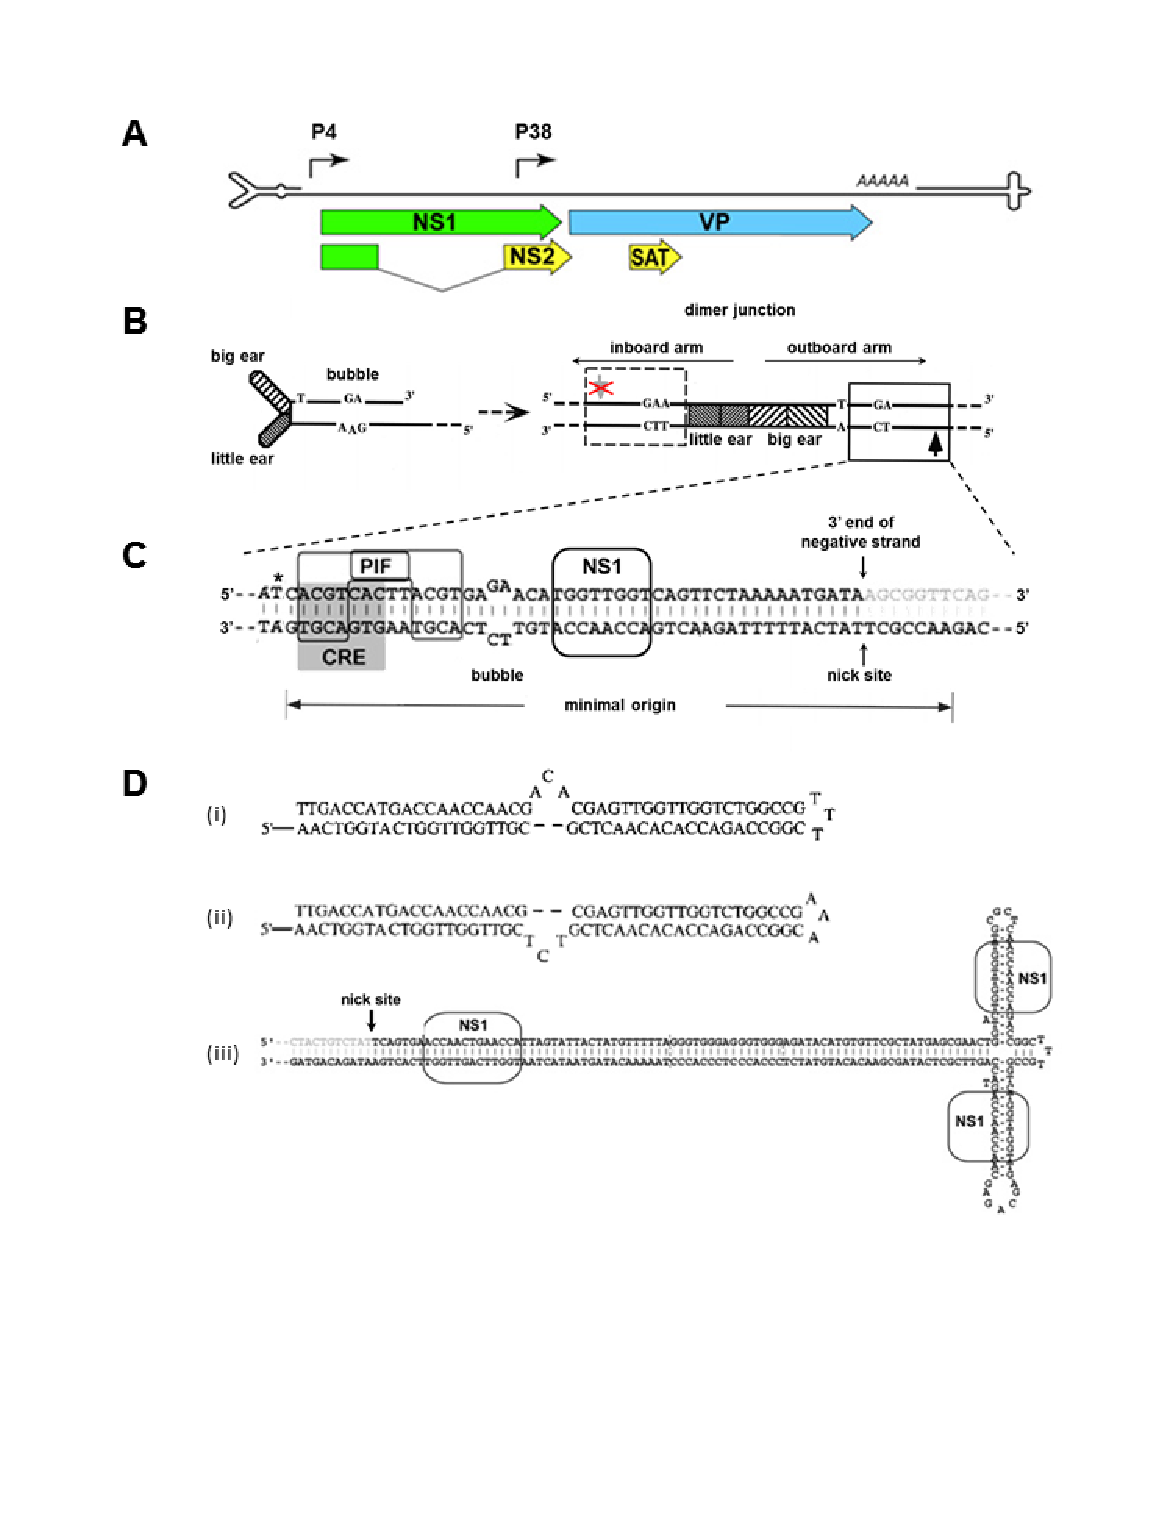
\includegraphics[scale=0.7]{Architecture}
  \vspace{-8em}
  \caption[Genome architecture of minute virus of mice (MVM).]
   {\textbf{(A)} The terminal hairpins, drawn to represent their predicted structures, are scaled approximately 20x relative to the rest of the genome. Major open reading frames are represented by arrowed boxes and alternative RNA splicing for NS2 is indicated. Proteins are shaded green for the major replication initiator protein (NS1), blue for the structural (VP) proteins of the capsid, and yellow for sequences unique to the ancillary nonstructural proteins. The two transcriptional promoters, P4 and P38, are indicated by rightward arrows and the polyadenylation site by the AAAAA-sequence block. Abbreviations: SAT, small alternatively translated protein \cite{small}. \textbf{(B)} The left-end hairpin of MVM and the dimer junction are shown in diagrammatic form. Asymmetries such as the "ear"-like structures, extra-helical T, and bubble sequence are indicated. The fully duplex, dimer junction, generated by rolling hairpin replication (see section~\ref{Replication}, p.~\pageref{Replication}), is shown on the right hand side. The short, palindromic sequences derived from the hairpin ears are represented by cross-hatched boxes. The active \textit{OriL\textsubscript{TC}} is boxed, with an arrow indicating the nick site. The equivalent sequence generated on the GAA side of the bubble is framed by a dashed box with an arrow at the potential nick site that is crossed out to indicate that \textit{OriL\textsubscript{GAA}} is not active \cite{pmid12885883, pmid16928767}. \textbf{(C)} Sequence details of the active left-end origin (approx. 50 bp) are shown, with an arrow indicating the active nick site. The minimal sequence required for origin activity is indicated by the double-headed arrow. Sequences of the bubble and the PIF, CRE, and NS1 binding sites are indicated. An asterisk represents the position of the extra-helical T, now base paired, and the gray box below it indicates the CRE consensus sequence \cite{pmid12885883}. \textbf{(D)} Alternate conformations of the right-end hairpin sequences of MVM. The right-end terminus can form a hairpin structure in either the flip (i) of flop (ii) sequence orientation or a cruciform structure (iii). In the cruciform configuration, the binding sites for the replicator protein, NS1, are boxed and their site of nucleolytic cleavage is represented by a vertical arrow \cite{pmid8614999}.
} 
\label{Architecture}
\end{figure}


\nomenclature{VP1}{Viral protein 1}
\nomenclature{VP2}{Viral protein 2}
\nomenclature{VP3}{Viral protein 3}
\nomenclature{NS}{Non-structural (protein)}
\nomenclature{PIF}{Parvovirus initiation factor}
\nomenclature{CRE}{cAMP-responsive element}
\nomenclature{SAT}{Small alternatively translated protein}

\subsection{Replication}
\label{Replication}
Due to the small capsid size of an approximate maximum external radius of 140 \r{A} \cite{pmid15299974}, the coding capacity of MVM genomic DNA is strictly limited. Consequently, the viral genes do not code for one's own DNA- and RNA polymerases and relevant accessory proteins. Thus, viral proliferation heavily depends on ancillary cellular factors that are essentially involved in viral genome replication and transcription. These factors are transiently supplied by proliferating host cells during the S-phase in the nucleus \cite{pmid16789120, pmid6602221, pmid3005655, pmid3296697, pmid9418888, pmid4673484, S-phase}. In contrast to other small, host cell depending DNA viruses, as for instance SV40 \cite{pmid4291013, pmid16578647}, MVM does not have the capability to stimulate resting cells and to initiate its DNA replication. Upon infection of resting host cells, MVM has to wait until infected cells enter S-phase of their own volition in order to amplify its DNA \cite{pmid4673484, pmid3346950, pmid10792046}.

Parvoviruses are unique among all known viruses in having a DNA genome that is both linear and single-stranded. Thus, it is not surprising that they evolutionary adapted their own one of a kind replication strategy. Their singular method to amplify the ssDNA genome resembles an ancient mechanism, known as rolling circle replication (RCR), that is utilized by many other small, circular prokaryotic and viral replicons \cite{pmid1630899, pmid8374079, pmid8824773, pmid9092519, pmid9010307}. However, in parvoviruses the RCR mechanism is modified and adapted for the replication of a linear chromosome. The parvoviral replication strategy, termed rolling hairpin replication (RHR), proceeds by a single-strand displacement mechanism, so there is no lagging-strand synthesis, and the integrity of the terminal hairpin sequences is maintained \cite{pmid967244}. The unidirectional progression of the replication fork results in the synthesis of a single, continuous DNA strand. In addition, MVM replication forks are aphidicolin-sensitive and require the proliferating cell nuclear antigen (PCNA). Such DNA elongation mechanism argues for a DNA synthesis that is mediated by DNA polymerase $\delta$ and its accessory proteins \cite{pmid10792046, pmid12050365}. 

In the initial stage of the RHR, complementary strand synthesis starts from the left-end snap-back telomere, which serves as a primer for the generation of double-stranded monomeric replicative form (mRF) DNA (see step (i) in figure~\ref{RHR}, p.~\pageref{RHR}). Subsequently, the growing complementary strand is ligated to the flipped-back right-end telomere by a host ligase, resulting in a covalently continuous RF (cRF) species (see step (ii) in figure~\ref{RHR}, p.~\pageref{RHR}) \cite{pmid2911112, pmid2543770}. This monomer-length turnaround intermediate functions as a transcription template for NS1 expression. NS1 is essential for all further stages of the RHR pathway because the cellular replication machinery is unable to melt, copy, and re-orient the left-end telomere \cite{pmid8995615}. In the first instance, NS1 nicks the right-end telomere (\textit{OriR}) of the cRF intermediate \cite{pmid9349487}, assisted by a host DNA-bending protein from the high-mobility group 1/2 (HMG 1/2) family (see step (iii) in figure~\ref{RHR}, p.~\pageref{RHR}) \cite{pmid9765384}. The resulting, liberated, 3' nucleotide at the nick site serves as a platform for the assembly of a new replication fork. NS1 remains covalently attached to the 5' end of the mRF DNA, where it functions as the 3' to 5' replicative helicase \cite{pmid12050365, pmid3339715, pmid3203742}. The next step (see step (iv) in figure~\ref{RHR}, p.~\pageref{RHR}), called "hairpin transfer", involves reopening and copying of the right-end hairpin sequence in order to generate a right-end extended duplex molecule, replacing the original sequence of the right-end telomere (R) with its inverted complement (r). The two previous steps (iii and iv) of the RHR are commonly referred to as "terminal resolution" \cite{telomere2}. In a NS1 dependent reaction, the extended duplex RF is melted and refolded into two hairpins, creating a "rabbit-ear" structure (see step (v) in figure~\ref{RHR}, p.~\pageref{RHR}) \cite{pmid14997524, pmid12075084}. In this way, the path of the replication fork is reversed effectively, redirecting it back along the internal coding sequences (see step (vi) in figure~\ref{RHR}, p.~\pageref{RHR}). Finally, this results in the generation of dimeric RF (dRF) and higher-order concatemeric molecules (see steps (vii-ix) in figure~\ref{RHR}, p.~\pageref{RHR}), in such a way that the viral coding sequence is replicated twice as frequently as the telomeres. Viral genomes are fused through a single palindromic junction, in either a left-end:left-end or right-end:right-end orientation. In a last step, individual, unit-length, ssDNA genomes are excised and displaced from the concatemeric RF intermediates. Initially, they feed back as new templates into the replicative pool to promote exponential DNA amplification but later they are consumed by encapsidation \cite{pmid15681430, encapsidation}.     

\cite{pmid967244, pmid3973977, pmid3296697, pmid8995615}         


\begin{figure}[t]
\centering
  \includegraphics[scale=0.7]{Replication}
  \caption[Rolling hairpin replication (RHR)]
   {Modified rolling hairpin model for MVM DNA replication. The sequence of the parvoviral genome is represented by a continuous line, colored blue for the parental genome, yellow for progeny genomes, and black for newly synthesized DNA, the 3’ end of which is capped by an arrowhead. The green sphere represents NS1, which nicks the covalently closed monomer (cRF) and remains attached to its 5’ end. The letters L and R depict the palindromic sequences at each terminus, with their inverted complements represented by l and r, respectively. Red dashed boxes depict the turnaround (tr) form of the right-end and the dimer junction (dJ) form of the left-end palindrome \cite{els}. 
} 
\label{RHR}
\end{figure}

\nomenclature{RCR}{Rolling circle replication}
\nomenclature{RHR}{Rolling hairpin replication}
\nomenclature{mRF}{Monomeric replicative form DNA}
\nomenclature{cRF}{Closed replicative form DNA}
\nomenclature{dRF}{Dimeric replicative form DNA}
\nomenclature{HMG 1/2}{High mobility group proteins 1 and 2}
\nomenclature{PCNA}{Proliferating cell nuclear antigen}

\subsection{Transcriptome}

\section{Viral proteins}


VP2...
The latter of which can be cleaved post-translationally by intracellular proteolytic cleavage to generate VP3, which displays a truncation of approximately 25 amino acids at its N-terminus \cite{pmid864702, pmid1448928, pmid9770425}. 


\subsection{Structural Proteins}

Three capsid proteins (LRV) \cite{pmid4321164}
Three capsid proteins (AAV) \cite{pmid5132697, pmid5172922}



\subsection{Non-structural proteins}
 
 \subsection{Packaging}
When the viral starnd is encapsidated, the terminal 24 bases attached to NS1 extend outside the capsid and can be subsequently cleaved off \cite{pmid2527311}.
%----------------------------------------------------------------------------------------

\section{}


\subsection{}



\subsection{}

